\hypertarget{sec:lrfk-results}{%
\section{Results}\label{sec:lrfk-results}}

Looking at the results of our MCMC simulations, we find a rich phase diagram with a CDW FTPT and interaction-tuned Anderson versus Mott localized phases similar to the 2D FK model~\autocite{antipovInteractionTunedAndersonMott2016}. We explore the localization properties of the fermionic sector and find that the localisation lengths vary dramatically across the phases and for different energies. Although moderate system sizes indicate the coexistence of localized and delocalized states within the CDW phase, we find quantitatively similar behaviour in a model of uncorrelated binary disorder on a CDW background. For large system sizes, i.e.~for our 1D disorder model we can treat linear sizes of several thousand sites, we find that all states are eventually localized with a localization length which diverges towards zero temperature.

\hypertarget{fig:phase-diagram-lrfk}{%
\begin{figure}
\centering
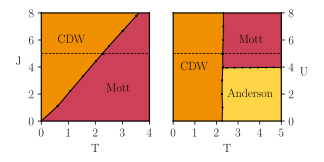
\includegraphics[width=1\textwidth,height=\textheight]{figure_code/fk_chapter/phase_diagram/phase_diagram}
\caption[{Long Range Falicov Kimball Model Phase Diagram}]{Phase diagrams of the long-range 1D FK model. (Left) The TJ plane at \(U = 5\): the CDW ordered phase is separated from a disordered Mott insulating phase by a critical temperature \(T_c\), linear in J. (Right) The TU plane at \(J = 5\): the disordered phase is split into two: at large/small U there's a MI/Anderson phase characterised by the presence/absence of a gap at \(E=0\) in the single particle energy spectrum. \(U_c\) is independent of temperature. At \(U = 0\) the fermions are decoupled from the spins forming a simple Fermi gas.}
\label{fig:phase-diagram-lrfk}
\end{figure}
}

\hypertarget{lrfk-results-phase-diagram}{%
\subsection{Phase Diagram}\label{lrfk-results-phase-diagram}}

Using the MCMC methods described in the previous section I will now discuss the results of extensive MCMC simulations of the model, starting with the phase diagram in the fermion spin coupling \(U\), the strength of the long range spin-spin coupling \(J\) and the temperature \(T\).

Fig \cref{fig:phase-diagram-lrfk} shows the phase diagram for constant \(U=5\) and constant \(J=5\), respectively. The transition temperatures were determined from the crossings of the Binder cumulants \(B_4 = \langle m^4 \rangle /\langle m^2 \rangle^2\)~\autocite{binderFiniteSizeScaling1981}.

The CDW transition temperature is largely independent from the strength of the interaction \(U\). This demonstrates that the phase transition is driven by the long-range term \(J\) with little effect from the coupling to the fermions \(U\). The physics of the spin sector in the long-range FK model mimics that of the long range Ising (LRI) model and is not significantly altered by the presence of the fermions. In two dimensions the transition to the CDW phase is mediated by an RKYY-like interaction~\autocite{rusinCalculationRKKYRange2017} but this is insufficient to stabilise long range order in one dimension. That the critical temperature \(T_c\) does not depend on \(U\) in our model further confirms this.

The main order parameters for this model is the staggered magnetisation \(m = N^{-1} \sum_i (-1)^i S_i\) that signals the onset of a charge density wave (CDW) phase at low temperature. However, my main interest concerns the additional structure of the fermionic sector in the high temperature phase. Following Ref.~\autocite{antipovInteractionTunedAndersonMott2016}, we can distinguish between the Mott and Anderson insulating phases. The Mott insulator is characterised by a gapped DOS in the absence of a CDW, instead the gap is driven entirely by interaction effect. Thus, the opening of a gap for large \(U\) is distinct from the gap-opening induced by the translational symmetry breaking in the CDW state below \(T_c\). The Anderson phase is gapless but, as we explain below, shows localised fermionic eigenstates hence it also has insulating character.

\hypertarget{localisation-properties}{%
\subsection{Localisation Properties}\label{localisation-properties}}

\hypertarget{fig:DOS}{%
\begin{figure}
\centering
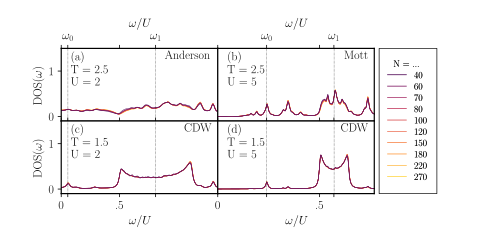
\includegraphics[width=1\textwidth,height=\textheight]{figure_code/fk_chapter/DOS/DOS}
\caption[{Energy resolved DOS(\(\omega\)) in the difference phases.}]{Energy resolved DOS(\(\omega\)) against system size \(N\) in all three phases. The charge density wave phase is shown in both the high and low \(U\) regime for completeness. The top left panel shows the Anderson phase at \(U = 2\) and high \(T = 2.5\), this phase is gapless but does not conduct due to Anderson localisation. In the lower left pane at \(U = 2\) and low \(T = 1.5\), charge density wave order sets in, allowing the single particle eigenstates to become extended but opening a gap in their band structure. In the upper right panel at \(U = 5\) and high \(T = 2.5\) the states are localised by disorder and an interaction driven gap opens, a Mott insulator. Finally the charge density wave phase at \(U = 5\) and \(T = 1.5\) is qualitatively similar to the lower left panel except that the gap scales with \(U\). For all the plots \(J = 5,\;\alpha = 1.25\).}
\label{fig:DOS}
\end{figure}
}

The MCMC formulation suggests viewing the spin configurations as a form of annealed binary disorder whose probability distribution is given by the Boltzmann weight \(e^{-\beta H_S[\vec{S}] - \beta F_c[\vec{S}]}\). This makes apparent the link to the study of disordered systems and Anderson localisation. While these systems are typically studied by defining the probability distribution for the quenched disorder potential externally, here we have a translation invariant system with disorder as a natural consequence of the Ising background field conserved under the dynamics.

In the limits of zero and infinite temperature, our model becomes a simple tight-binding model for the fermions. At zero temperature, the spin background is in one of the two translation invariant AFM ground states with two gapped fermionic CDW bands at energies \[E_{\pm} = \pm\sqrt{\frac{1}{4}U^2 + 2t^2(1 + \cos ka)^2}\;.\]

At infinite temperature, all the spin configurations become equally likely and the fermionic model reduces to one of binary uncorrelated disorder in which all eigenstates are Anderson localised~\autocite{abrahamsScalingTheoryLocalization1979}. An Anderson localised state centered around \(r_0\) has magnitude that drops exponentially over some localisation length \(\xi\) i.e \(|\psi(r)|^2 \sim \exp{-|r - r_0|/\xi}\). Calculating \(\xi\) directly is numerically demanding. Therefore, we determine if a given state is localised via the energy-resolved IPR and the DOS defined as \[\begin{aligned}
\mathrm{DOS}(\vec{S}, \omega)& = N^{-1} \sum_{i} \delta(\epsilon_i - \omega)\\
\mathrm{IPR}(\vec{S}, \omega)& = \; N^{-1} \mathrm{DOS}(\vec{S}, \omega)^{-1} \sum_{i,j} \delta(\epsilon_i - \omega)\;\psi^{4}_{i,j}\end{aligned}\] where \(\epsilon_i\) and \(\psi_{i,j}\) are the \(i\)th energy level and \(j\)th element of the corresponding eigenfunction, both dependent on the background spin configuration \(\vec{S}\).

\hypertarget{fig:IPR_scaling}{%
\begin{figure}
\centering
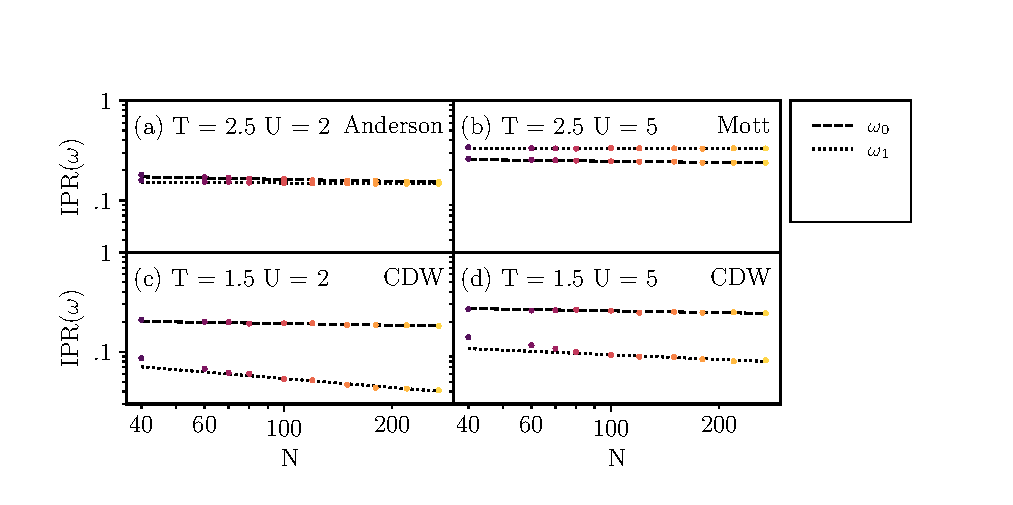
\includegraphics[width=1\textwidth,height=\textheight]{figure_code/fk_chapter/DOS/IPR_scaling}
\caption[{Scaling of IPR(\(\omega\)) against system size \(N\).}]{The IPR(\(\omega\)) scaling with \(N\) at fixed energy for each phase and for points both in the gap (\(\omega_0\)) and in a band (\(\omega_1\)). The slope of the line yields the scaling exponent \(\tau\) defined by \(\mathrm{IPR} \propto N^{-\tau}\)). \(\tau\) close to zero implies that the states at that energy are localised while \(\tau = -d\) corresponds to extended states where \(d\) is the system dimension. All but the bands of the charge density wave phase are approximately localised with \(\tau\) is very close to zero. The bands in the charge density wave phase are localised with long localisation lengths at finite temperatures that extend to infinity as the temperature approaches zero. For all the plots \(J = 5,\;\alpha = 1.25\). The measured \(\tau_0,\tau_1\) for each figure are: (a) \((0.06\pm0.01, 0.02\pm0.01\) (b) \(0.04\pm0.02, 0.00\pm0.01\) (c) \(0.05\pm0.03, 0.30\pm0.03\) (d) \(0.06\pm0.04, 0.15\pm0.05\) We show later that the apparent slight scaling of the IPR with system size in the localised cases can be explained by finite size effects due to the changing defect density with system size rather than due to delocalisation of the states.}
\label{fig:IPR_scaling}
\end{figure}
}

The scaling of the IPR with system size

\[\mathrm{IPR} \propto N^{-\tau}\]

depends on the localisation properties of states at that energy. For delocalised states, e.g.~Bloch waves, \(\tau\) is the physical dimension. For fully localised states \(\tau\) goes to zero in the thermodynamic limit. However, for special types of disorder such as binary disorder, the localisation lengths can be large comparable to the system size at hand, which can make it difficult to extract the correct scaling. An additional complication arises from the fact that the scaling exponent may display intermediate behaviours for correlated disorder and in the vicinity of a localisation-delocalisation transition~\autocite{kramerLocalizationTheoryExperiment1993,eversAndersonTransitions2008}. The thermal defects of the CDW phase lead to a binary disorder potential with a finite correlation length, which in principle could result in delocalized eigenstates.

The key question for our system is then: How is the \(T=0\) CDW phase with fully delocalized fermionic states connected to the fully localized phase at high temperatures?

For a representative set of parameters covering all three phases \cref{fig:DOS} shows the density of states as function of energy while \cref{fig:IPR_scaling}~shows \(\tau\), the scaling exponent of the IPR with system size, The DOS is symmetric about \(0\) because of the particle hole symmetry of the model. At high temperatures, all of the eigenstates are localised in both the Mott and Anderson phases (with \(\tau \leq 0.07\) for our system sizes). We also checked that the states are localised by direct inspection. Note that there are in-gap states for instance at \(\omega_0\), below the upper band which are localized and smoothly connected across the phase transition.

\hypertarget{fig:gap_opening_U5}{%
\begin{figure}
\centering
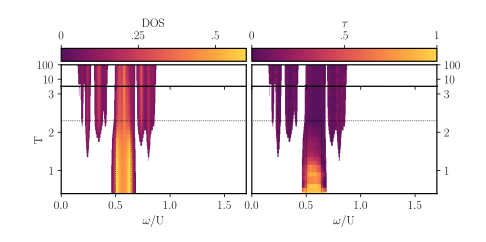
\includegraphics[width=1\textwidth,height=\textheight]{figure_code/fk_chapter/gap_opening/gap_opening_U5}
\caption[{The transition from CDW to the Mott phase}]{The DOS (a) and scaling exponent \(\tau\) (b) as a function of energy for the CDW to gapped Mott phase transition at \(U=5\). Regions where the DOS is close to zero are shown in white. The scaling exponent \(\tau\) is obtained from fits to \(IPR(N) = A N^{-\lambda}\) for a range of system sizes. \(J = 5,\;\alpha = 1.25\)}
\label{fig:gap_opening_U5}
\end{figure}
}

In the CDW phases at \(U=2\) and \(U=5\), we find for the states within the gapped CDW bands, e.g.~at \(\omega_1\), scaling exponents \(\tau = 0.30\pm0.03\) and \(\tau = 0.15\pm0.05\), respectively. This surprising finding suggests that the CDW bands are partially delocalised with multi-fractal behaviour of the wavefunctions~\autocite{eversAndersonTransitions2008}. This phenomenon would be unexpected in a 1D model as they generally do not support delocalisation in the presence of disorder except as the result of correlations in the emergent disorder potential~\autocite{croyAndersonLocalization1D2011,goldshteinPurePointSpectrum1977}. However, we later show by comparison to an uncorrelated Anderson model that these nonzero exponents are a finite size effect and the states are localised with a finite \(\xi\) similar to the system size, an example of weak localisation. As a result, the IPR does not scale correctly until the system size has grown much larger than \(\xi\). \cref{fig:DM_IPR_scaling} shows that the scaling of the IPR in the CDW phase does flatten out eventually.

Next, we use the DOS and the scaling exponent \(\tau\) to explore the localisation properties over the energy-temperature plane in \cref{fig:gap_opening_U2} and \cref{fig:gap_opening_U5}. Gapped areas are shown in white, which highlights the distinction between the gapped Mott phase and the ungapped Anderson phase. In-gap states appear just below the critical point, smoothly filling the bandgap in the Anderson phase and forming islands in the Mott phase. As in the finite~\autocite{zondaGaplessRegimeCharge2019} and infinite dimensional~\autocite{hassanSpectralPropertiesChargedensitywave2007} cases, the in-gap states merge and are pushed to lower energy for decreasing U as the \(T=0\) CDW gap closes. Intuitively, the presence of in-gap states can be understood as a result of domain wall fluctuations away from the AFM ordered background. These domain walls act as local potentials for impurity-like bound states~\autocite{zondaGaplessRegimeCharge2019}.

\hypertarget{fig:gap_opening_U2}{%
\begin{figure}
\centering
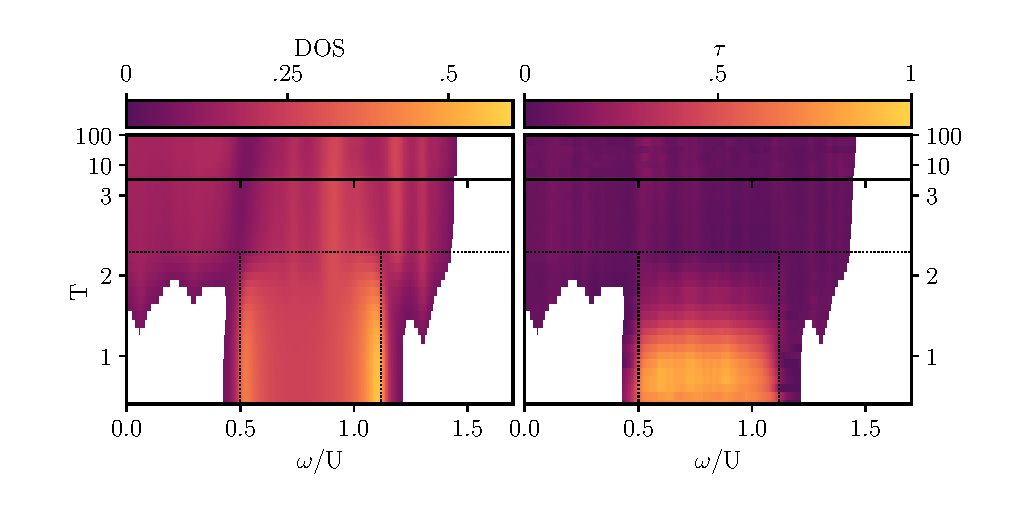
\includegraphics[width=1\textwidth,height=\textheight]{figure_code/fk_chapter/gap_opening/gap_opening_U2}
\caption[{The transition from CDW to the Anderson Phase}]{The DOS (a) and scaling exponent \(\tau\) (b) as a function of energy for the CDW phase to the gapless Anderson insulating phase at \(U=2\). Regions where the DOS is close to zero are shown in white. The scaling exponent \(\tau\) is obtained from fits to \(IPR(N) = A N^{-\lambda}\) for a range of system sizes. \(J = 5,\;\alpha = 1.25\)}
\label{fig:gap_opening_U2}
\end{figure}
}

In order to understand the localization properties we can compare the behaviour of our model with that of a simpler Anderson disorder model (DM) in which the spins are replaced by a CDW background with uncorrelated binary defect potentials. This is defined by replacing the spin degree of freedom in the FK model \(S_i = \pm \tfrac{1}{2}\) with a disorder potential \(d_i = \pm \tfrac{1}{2}\) controlled by a defect density \(\rho\) such that \(d_i = -\tfrac{1}{2}\) with probability \(\rho/2\) and \(d_i = \tfrac{1}{2}\) otherwise. \(\rho/2\) is used rather than \(\rho\) so that the disorder potential takes on the zero temperature CDW ground state at \(\rho = 0\) and becomes a random choice over spin states at \(\rho = 1\) i.e the infinite temperature limit.

\[\begin{aligned}
H_{\mathrm{DM}} = & \;U \sum_{i} (-1)^i \; d_i \;(c^\dagger_{i}c_{i} - \tfrac{1}{2}) \\
& -\;t \sum_{i} c^\dagger_{i}c_{i+1} + c^\dagger_{i+1}c_{i}
\end{aligned}\]

\cref{fig:DM_DOS} and \cref{fig:DM_IPR_scaling} compare the FK model to the disorder model at different system sizes, matching the defect densities of the disorder model to the FK model at \(N = 270\) above and below the CDW transition. We find very good, even quantitative, agreement between the FK and disorder models, which suggests that correlations in the spin sector do not play a significant role.

\hypertarget{fig:DM_DOS}{%
\begin{figure}
\centering
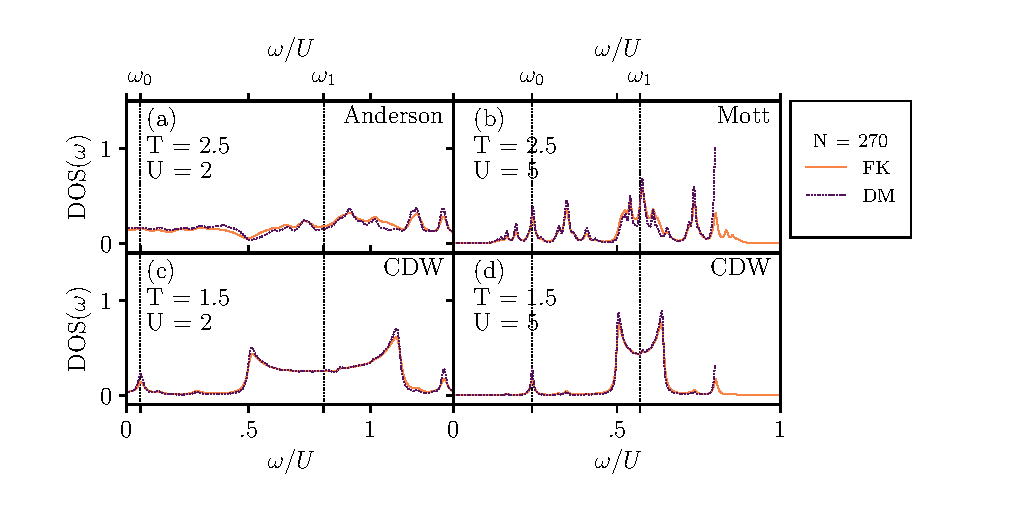
\includegraphics[width=1\textwidth,height=\textheight]{figure_code/fk_chapter/disorder_model/DM_DOS}
\caption[{FK model compared to binary disorder model: DOS}]{A comparison of the full FK model to a simple binary disorder model (DM) with a CDW wave background perturbed by uncorrelated defects at density \(0 < \rho < 1\) matched to the \(\rho\) for the largest corresponding FK model. As in \cref{fig:DOS}, the Energy resolved DOS(\(\omega\)) is shown. The DOSs match well implying that correlations in the CDW wave fluctuations are not relevant at these system parameters.}
\label{fig:DM_DOS}
\end{figure}
}

As we can sample directly from the disorder model, rather than through MCMC, the samples are uncorrelated. Hence we can evaluate much larger system sizes with the disorder model which enables us to pin down the correct localisation effects. In particular, what appear to be delocalized states for small system sizes eventually turn out to be states with large localization length. The localization length diverges towards the ordered zero temperature CDW state. The interplay of interactions, which here produce as peculiar binary potential, and localization can be very intricate and the added advantage of a 1D model is that we can explore very large system sizes.

\hypertarget{fig:DM_IPR_scaling}{%
\begin{figure}
\centering
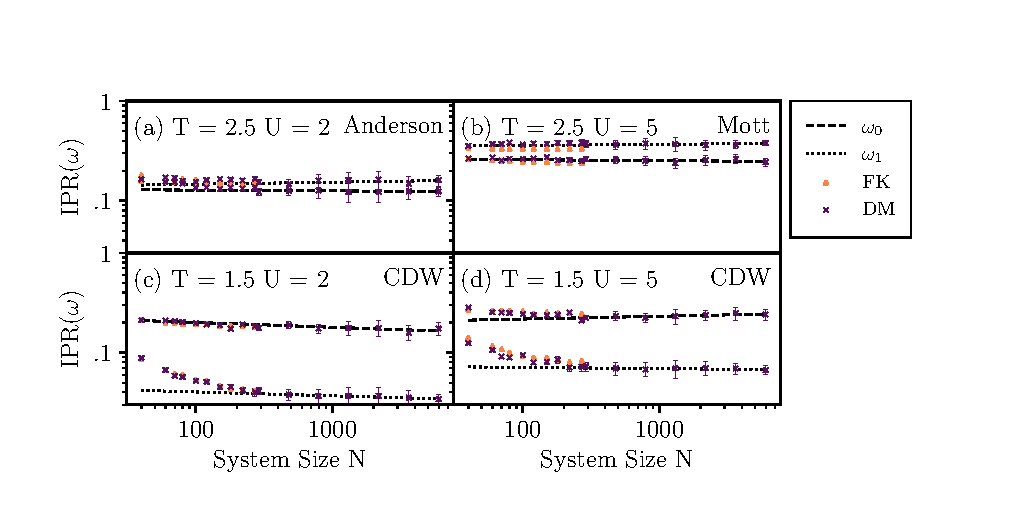
\includegraphics[width=1\textwidth,height=\textheight]{figure_code/fk_chapter/disorder_model/DM_IPR_scaling}
\caption[{FK model compared to binary disorder model: IPR Scaling}]{A comparison of the full FK model to a simple binary disorder model (DM) with a CDW wave background perturbed by uncorrelated defects at density \(0 < \rho < 1\) matched to the \(\rho\) for the largest corresponding FK model. As in \cref{fig:IPR_scaling} \(\tau(\omega)\) the scaling of IPR(\(\omega\)) with system size, , is shown both in gap (\(\omega_0\)) and in the band (\(\omega_1\)). This data makes clear that the apparent scaling of IPR with system size at small sysis a finite size effect due to weak localisation~\autocite{antipovInteractionTunedAndersonMott2016}, hence all the states are indeed localised as one would expect in 1D. The disorder model \(\tau_0,\tau_1\) for each figure are: (a) \(0.01\pm0.05, -0.02\pm0.06\) (b) \(0.01\pm0.04, -0.01\pm0.04\) (c) \(0.05\pm0.06, 0.04\pm0.06\) (d) \(-0.03\pm0.06, 0.01\pm0.06\). The lines are fit on system sizes \(N > 400\)}
\label{fig:DM_IPR_scaling}
\end{figure}
}

\hypertarget{fk-conclusion}{%
\section{Discussion and Conclusion}\label{fk-conclusion}}

The FK model is one of the simplest non-trivial models of interacting fermions. We studied its thermodynamic and localisation properties brought down in dimensionality to one dimension by adding a novel long-ranged coupling designed to stabilise the CDW phase present in dimension two and above.

Our MCMC approach emphasises the presence of a disorder-free localization mechanism within our translationally invariant system. Further, it gives a significant speed up over the naive method. We show that our LRFK model retains much of the rich phase diagram of its higher dimensional cousins. Careful scaling analysis indicates that all the single particle eigenstates eventually localise at non-zero temperature albeit only for very large system sizes of several thousand.

Our work raises a number of interesting questions for future research. A straightforward but numerically challenging problem is to pin down the model's behaviour closer to the critical point where correlations in the spin sector would become significant. Would this modify the localisation behaviour? Similar to other soluble models of disorder-free localisation, we expect intriguing out-of equilibrium physics, for example slow entanglement dynamics akin to more generic interacting systems~\autocite{hartLogarithmicEntanglementGrowth2020}. One could also investigate whether the rich ground state phenomenology of the FK model as a function of filling~\autocite{gruberGroundStatesSpinless1990} such as the devil's staircase~\autocite{michelettiCompleteDevilTextquotesingles1997} as well as superconductor like states~\autocite{caiVisualizingEvolutionMott2016} could be stabilised at finite temperature.

In a broader context, we envisage that long-range interactions can also be used to gain a deeper understanding of the temperature evolution of topological phases. One example would be a long-ranged FK version of the celebrated Su-Schrieffer-Heeger model where one could explore the interplay of topological bound states and thermal domain wall defects. Finally, the rich physics of our model should be realizable in systems with long-range interactions, such as trapped ion quantum simulators, where one can also explore the fully interacting regime with a dynamical background field.
